\documentclass{standalone}
\usepackage{tikz}
\begin{document}
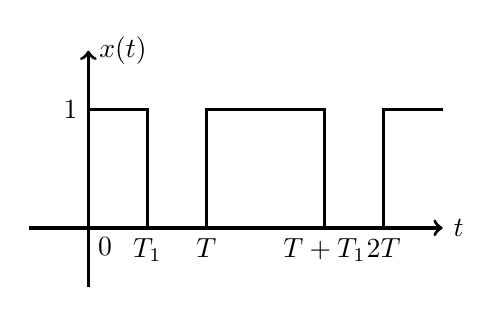
\begin{tikzpicture}[scale=1.5]
    \draw[->,very thick](-0.5,0)--(3,0)node[right]{$t$};
    \draw[->,very thick](0,-0.5)--(0,1.5)node[right]{$x(t)$};
    \node[below right]at(0,0){$0$};

    \draw[-,very thick](0,1)node[left]{$1$}--(0.5,1)--(0.5,0)node[below]{$T_1$}--(1,0)node[below]{$T$}--(1,1)--(2,1)--(2,0)node[below]{$T+T_1$}--(2.5,0)node[below]{$2T$}--(2.5,1)--(3,1);
\end{tikzpicture}
\end{document}